%%________________________________________________________________________
%% LEIM | PROJETO
%% 2022 / 2013 / 2012
%% Modelo para relat�rio
%% v04: altera��o ADEETC para DEETC; outros ajustes
%% v03: corre��o de gralhas
%% v02: inclui anexo sobre utiliza��o sistema controlo de vers�es
%% v01: original
%% PTS / MAR.2022 / MAI.2013 / 23.MAI.2012 (constru�do)
%%________________________________________________________________________




%%________________________________________________________________________
\chapter{Um Detalhe Adicional}
\label{ch:umDetalheAdicional}
%%________________________________________________________________________

O \aspas{ap�ndice} utiliza-se para descrever aspectos que tendo sido desenvolvidos pelo autor constituem um complemento ao que j� foi apresentado no corpo principal do documento.

Neste documento utilize o ap�ndice para explicar o processo usado na \textbf{gest�o das vers�es} que foram sendo constru�das ao longo do desenvolvimento do trabalho.

� especialmente importante explicar o objetivo de cada ramo (\aspas{branch}) definido no projeto (ou apenas dos ramos mais importantes) e indicar quais os ramos que participaram numa jun��o (\aspas{merge}).

� tamb�m importante explicar qual a arquitetura usada para interligar os v�rios reposit�rios (\eg, Git, GitHub, DropBox, GoogleDrive) que cont�m as v�rias vers�es (e respetivos ramos) do projeto.


Notar a diferen�a essencial entre \aspas{ap�ndice} e \aspas{anexo}. O \aspas{ap�ndice} � um texto (ou documento) que descreve trabalho desenvolvido pelo autor (\eg, do relat�rio, monografia, tese). O \aspas{anexo} � um texto (ou documento) sobre trabalho que n�o foi desenvolvido pelo autor.

Para simplificar vamos apenas considerar a no��o de \aspas{ap�ndice}. No entanto, pode sempre adicionar os anexos que entender como adequados.






%%________________________________________________________________________
\chapter{Outro Detalhe Adicional}
\label{ch:outroDetalheAdicional}
%%________________________________________________________________________

\begin{figure}[h]
   \centering
   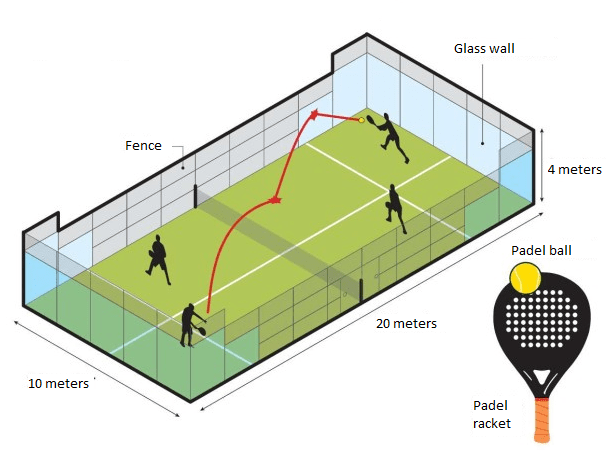
\includegraphics[width=12cm]{./padel_court}
\caption{Descri��o pormenorizada do campo de padel. \cite{tennisnerd_padel_2019}}
\label{fig:campopadel}
\end{figure}












